\section{Evaluation}
To demonstrate the efficacy of our method, we first fit Equation~\ref{eq:RS} using a well known rating system, the Sagarin ratings.  Then, $\rho$ is calibrated based on historical results from the previous seven years NCAA tournaments.  Note seven years was chosen as this is the complete history of the team and player level characterstics used to find neighbors of teams.   The log loss for 2014 for the entire range of $\rho$ can be seen in Figure~\ref{fig:result} and the value that was selected based on historical results $0.2$.
\begin{figure}[h]
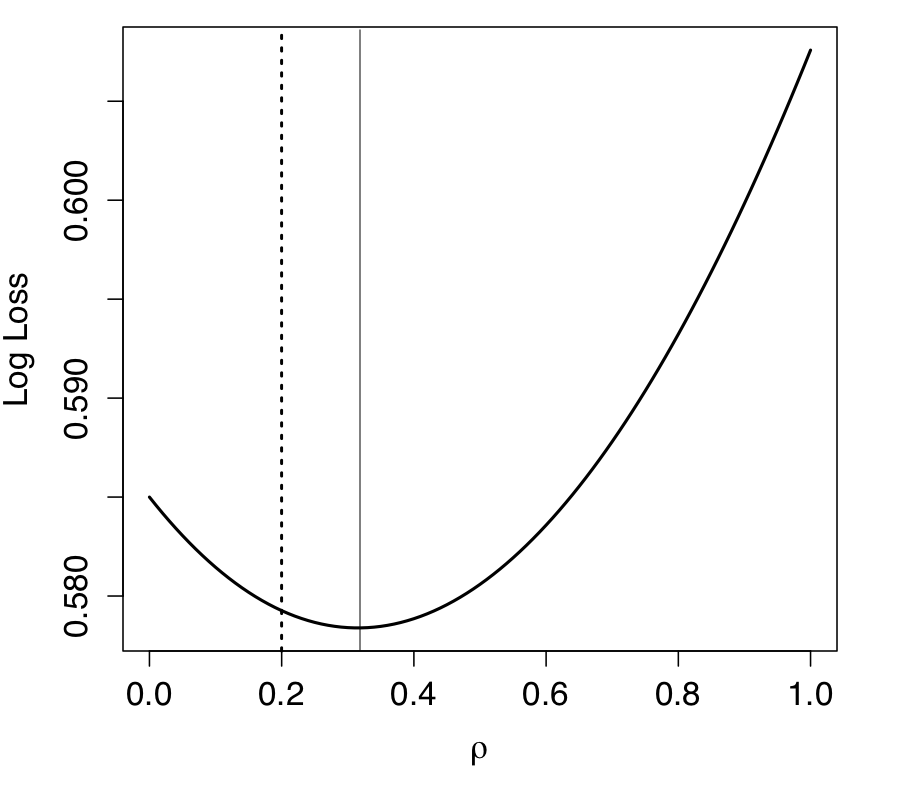
\includegraphics[width=1\textwidth]{results_2014.png}
\caption{Log loss for no matchup effect = red, log loss for optimized $\rho$ = blue}
\label{fig:result}
\end{figure}

The selected $\rho$ value results in a reduction in loss.  A modest gain is also seen in classification error from (0.365 to 0.350) although this is only a single game difference.  The matchup effect, particularly with smaller $\rho$ values, will have a lesser effect on classification error than that off the loss functions like the log loss.  This is because it will only shift the expected point differential a fairly small margin, so the only games in which classification error would change are those that are nearly dead heat games to begin with.

To illustrate the matchup effects, consider Table~\ref{tab:change} which contains the ten games that saw the largest shift in expected point differential.  This table contains expected point differentials (team1 - team2) and probabilities of team 1 winning under a standard relative strength model using the Sagarin ratings as well as the adjusted results using the Nearest Neighbor Matchup Effects.  The table also contains the realized loss for the each resulting game.
\begin{table}[ht]
\caption{Ten games with largest point differential change}
\footnotesize
\centering
\begin{tabular}{|cc | ccc | ccc | c|}
  \hline
  \hline
 team 1 & team 2 & Point Diff & Prob & Loss & Point Diff:ME & Prob:ME & Loss:ME & winning team \\ 
  \hline
 Cal Poly & Wichita St & -18.69 & 0.04 & 0.04 & -17.10 & 0.06 & 0.06 & Wichita St \\ 
 Connecticut & St. Joseph's &4.29 & 0.65 & 0.43 & 6.18 & 0.71 & 0.34 & Connecticut \\ 
 Dayton & Stanford & -2.16 & 0.42 & 0.86 & 0.94 & 0.53 & 0.63 & Dayton \\ 
 Dayton & Syracuse & -6.34 & 0.28 & 1.27 & -4.05 & 0.36 & 1.03 & Dayton \\ 
 Kentucky & Michigan & -3.71 & 0.37 & 1.00 & -2.08 & 0.42 & 0.86 & Kentucky \\ 
 UMass & Tennessee &-3.05 & 0.39 & 0.49 & -4.83 & 0.33 & 0.40 & Tennessee \\ 
 Memphis & Virginia & -6.34 & 0.28 & 0.33 & -8.91 & 0.21 & 0.23 & Virginia  \\ 
 Michigan & Tennessee & 5.37 & 0.69 & 0.37 & 3.49 & 0.62 & 0.47 & Michigan\\ 
 Michigan & Texas & 8.05 & 0.77 & 0.26 & 5.85 & 0.70 & 0.35 & Michigan \\ 
 Syracuse & W. Michigan & 12.65 & 0.88 & 0.13 & 15.01 & 0.92 & 0.09 & Syracuse \\ 
   \hline
   \hline
\end{tabular}
\label{tab:change}
\end{table}
On this particular subset of games, the matchup effects model performs considerably better than the typical model under the log loss (.446 to .520).  As the other games see minimal matchup effects, the results are essentially the same.  